% !TeX root=main.tex

\section{Methodik der Thesis}

Die Methodik dieser Bachelorarbeit basiert auf einer Kombination aus einer Literaturrecherche und Fallstudienanalyse. Diese Methodenkombination ermöglicht es, ein fundiertes theoretisches Fundament zu legen und gleichzeitig praktische Einblicke zu gewinnen, um die Forschungsfragen zu beantworten.

\begin{figure}[H]
    \centering
    \caption{Aufbau und Struktur der Bachelorthesis mit Forschungsmethodik}
    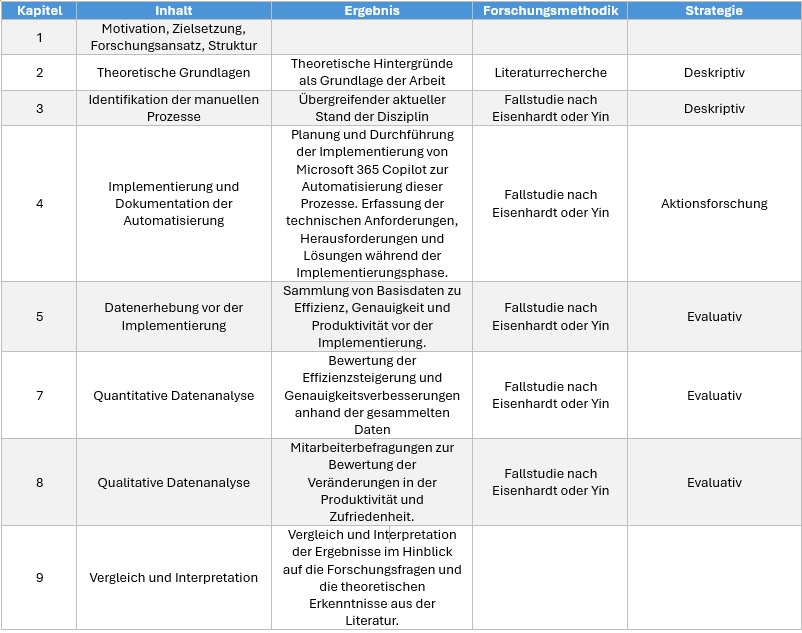
\includegraphics[scale=0.6]{methodik}
    \captionsetup{font=scriptsize}
    \label{fig:methodik}
\end{figure}

Die Methodik der Fallstudienforschung basiert auf bewährten Ansätzen der Design Science Research (DSR) von Shirley und Hevner\footnote{Vgl. \cite{Shirley&Hevner2013}, S.337-355}. DSR ist ein strukturierter Ansatz innovative Artefakte zu entwickeln und die Relevanz in realen Anwendungsszenarien zu evualieren. Wie in der Abbildung \ref{fig:methodik} dargestellt besteht die Fallstudienforschung aus Problemidentifikation, Zieldefinition, Entwicklung, Implementierung und Dokumentation. Die qualitative Datenerhebung erfolgt über Expertengespräche mit einer systematischen Vorgehensweise und Analyse nach Mayring\footnote{Vgl. \cite{Mayring2019}, S.633-648}. 

Die Methodik der Literaturrecherche basiert auf dem Ansatz von Brocke et al.\footnote{Vgl. \cite{Brocke2015}, S. 205-224} und wurde bereits begonnen. Die Literaturrecherche wurde auf folgenden Plattformen durchgeführt:

\begin{itemize}
    \item IEEE Xplore: \underline{\textcolor{blue}{https://ieeexplore.ieee.org/}}
    \item Science Direkt: \underline{\textcolor{blue}{https://www.sciencedirect.com/}}
    \item Google Scholar: \underline{\textcolor{blue}{https://scholar.google.com/}}
    \item Springer Link: \underline{\textcolor{blue}{https://link.springer.com/}}
\end{itemize}

Die Tabelle \ref{table:search_results} beschreibt die Suchalgorithmen in den jeweiligen Plattformen mit der Anzahl der Treffer und des ausgewählten Journalartikels. Der H-Index wird als Qualitätsmerkmal der Journals dargestellt.\footnote{Vgl. \cite{Bornmann2007}, S. 1381-1385} Das Q-Ranking wird aus dem Onlineportal SCImago Journal Rank (SJR)\footnote{Vgl. https://www.scimagojr.com/countryrank.php } entnommen, sortiert die Journals in regionale Kategorien und wird für die Auswahl als Qualitätsmerkmal verwendet. Nicht für alle Journals konnte ein H-Index oder Q-Ranking ermittelt werden, da die Daten zu den ermittelten Journals nicht vollständig verfügbar waren.

Die Suchalgorithmen wurden so konzipiert, dass sie die relevantesten Artikel zu den Themen ''Business Intelligence'', ''Large Language Models'', ''Copilot'' und ''Automatisierung'' identifizieren. Die Algorithmen wurden kontinuierlich angepasst, um eine möglichst geringe Trefferanzahl zu erhalten. Die Auswahl der Journalartikel erfolgte anhand der Relevanz für die Forschungsfragen und der Qualität der Quellen. Der Verlauf der Literaturrecherche wird in der Tabelle \ref{table:search_results} dargestellt.

\begin{scriptsize}
\begin{longtable}{|p{1cm}|p{3cm}|C{1.1cm}|p{4cm}|c|C{1.2cm}|}
    \caption{Systematische Literaturrecherche} \label{table:search_results} \\
    \hline
    \textbf{Suchort} & \textbf{Suchalgorithmus} & \textbf{Anzahl Treffer} & \textbf{Auswahl} & \textbf{H-Index} & \textbf{Q-Ranking} \\
    \hline
    IEEE Xplore & ((''Business Intelligence'' AND ''large language models'') OR ((''business'' AND ''intelligence'') AND ''large language models'')) & 6 & M. A. K. Raiaan et al., ''A Review on Large Language Models: Architectures, Applications, Taxonomies, Open Issues and Challenges,'' in IEEE Access, vol. 12, pp. 26839-26874, 2024 & 242 & Q1 \\
    \hline
    IEEE Xplore & ((''Business Intelligence'' AND ''large language models'') OR ((''business'' AND ''intelligence'') AND ''large language models'')) & 6 & Z. Wang, ''Empowering Few-Shot Recommender Systems With Large Language Models-Enhanced Representations,'' in IEEE Access, vol. 12, pp. 29144-29153, 2024 & 242 & Q1 \\
    \hline
    IEEE Xplore & ((''Business Intelligence'' AND ''large language models'') OR ((''business'' AND ''intelligence'') AND ''large language models'')) & 6 & A. Ghandour, B. J. Woodford and H. Abusaimeh, ''Ethical Considerations in the Use of ChatGPT: An Exploration Through the Lens of Five Moral Dimensions,'' in IEEE Access, vol. 12, pp. 60682-60693, 2024 & 242 & Q1 \\
    \hline
    Science Direkt & (((''Business Intelligence'' AND (''large language model'') AND (''automate'' OR ''automatize'')) OR ((''business intelligence'') and (''large language model'') AND (''automate'' OR ''automatize'')))) & 31 & Abram Handler, Kai R. Larsen, Richard Hackathorn, Large language models present new questions for decision support, International Journal of Information Management,Volume 79,2024 & 177 & Q1 \\
    \hline
    Science Direkt & ((''Business Intelligence'' AND (''large language model'') AND (''automate'' OR ''automatize'')) OR ((''business intelligence'') and (''large language model'') AND (''automate'' OR ''automatize''))) & 31 & Robert Buchmann, Johann Eder, Hans-Georg Fill, Ulrich Frank, Dimitris Karagiannis, Emanuele Laurenzi, John Mylopoulos, Dimitris Plexousakis, Maribel Yasmina Santos,Large language models: Expectations for semantics-driven systems engineering,Data \& Knowledge Engineering,Volume 152,2024 & 94 & Q2 \\
    \hline
    Science Direkt & ((''Business Intelligence'' AND (''large language model'') AND (''automate'' OR ''automatize'')) OR ((''business intelligence'') and (''large language model'') AND (''automate'' OR ''automatize''))) & 31 & Adel Remadi, Karim El Hage, Yasmina Hobeika, Francesca Bugiotti,To prompt or not to prompt: Navigating the use of Large Language Models for integrating and modeling heterogeneous data,Data \& Knowledge Engineering,Volume 152,2024 & 94 & Q2 \\
    \hline
    Science Direkt & ((''Business Intelligence'' AND (''large language model'') AND (''automate'' OR ''automatize'')) OR ((''business intelligence'') and (''large language model'') AND (''automate'' OR ''automatize''))) & 181 & Pradnya Sawant, Kavita Sonawane,NLP-based smart decision making for business and academics,Natural Language Processing Journal,2024 & - & - \\
    \hline
    Google Scholar & ((''Business Intelligence'' AND (''large language model'') AND (''automate'' OR ''automatize'')) OR ((''business intelligence'') and (''large language model'') AND (''automate'' OR ''automatize''))) & 181 & Sobhkhiz, S., \& El-Diraby, T. Natural Language Processing for Building Maintenance: From Deep Learning to Business Intelligence. Available at SSRN 4783740. & - & - \\
    \hline
    Google Scholar & ((''Business Intelligence'' AND (''large language model'') AND (''automate'' OR ''automatize'')) OR ((''business intelligence'') and (''large language model'') AND (''automate'' OR ''automatize''))) & 181 & TSAO, Wen-Kwang. Multi-agent reasoning with large language models for effective corporate planning. In: 2023 International Conference on Computational Science and Computational Intelligence (CSCI). IEEE, 2023. S. 365-370. & - & - \\
    \hline
    Google Scholar & ((''Business Intelligence'' AND (''large language model'') AND (''automate'' OR ''automatize'')) OR ((''business intelligence'') and (''large language model'') AND (''automate'' OR ''automatize''))) & 181 & KUMAR, Sandeep; VANDANAPU, Manoj Kumar. Natural Language Generation and Artificial Intelligence in Financial Reporting: Transforming Financial Data into Strategic Insights for Executive Leadershi (IJCET), 2024, 15. Jg., Nr. 2. & 16 & Q4 \\
    \hline
    Springer Link & ((''Business Intelligence'' AND (''large language model'') AND (''automate'' OR ''automatize'')) OR ((''business intelligence'') and (''large language model'') AND (''automate'' OR ''automatize''))) & 7 & Khtar, Z.B. Unveiling the evolution of generative AI (GAI): a comprehensive and investigative analysis toward LLM models (2021–2024) and beyond. Journal of Electrical Systems and Inf Technol 11, 22 (2024) & - & - \\
    \hline
    IEEE Xplore & ((''Copilot'') AND (''case study'')) & 2 & Z. Ságodi, I. Siket and R. Ferenc, ''Methodology for Code Synthesis Evaluation of LLMs Presented by a Case Study of ChatGPT and Copilot,'' in IEEE Access, vol. 12, pp. 72303-72316, 2024 & 62 & Q2 \\
    \hline
    IEEE Xplore & ((Business Intelligence'') AND (''large language model'' OR ''LLM'' OR ''NLP'' OR ''Natural Language Processing'')) & 7 & B. K. Chae, ''Big Data and IT-Enabled Services: Ecosystem and Coevolution,'' in IT Professional, vol. 17, no. 2, pp. 20-25, Mar.-Apr. 2015 & 242 & Q1 \\
    \hline
    IEEE Xplore & ((''Microsoft'') OR (''Copilot'')) AND ((''large language model'') OR (''LLM'')) & 5 & C. Wang, J. Thompson and B. Lee, ''Data Formulator: AI-Powered Concept-Driven Visualization Authoring,'' in IEEE Transactions on Visualization and Computer Graphics, vol. 30, no. 1, pp. 1128-1138, Jan. 2024 & 166 & Q1 \\
    \hline
    IEEE Xplore & ((''Microsoft'') OR (''Copilot'')) AND ((''large language model'') OR (''LLM'')) & 5 & C. Shi et al., ''NL2Color: Refining Color Palettes for Charts with Natural Language'', in IEEE Transactions on Visualization and Computer Graphics, Bd. 30, Nr. 1, S. 814-824, Jan. 2024 & 166 & Q1 \\
    \hline
\end{longtable}
\end{scriptsize}

\clearpage